\section{Model-based Testing}\label{sec:model_based_testing}

Model-based testing is a testing technique where a System Under Test (SUT) is tested for conformance to a model description of the system. The general setup for this process is depicted in Figure~\ref{fig:model_based_testing}. The specification of a system, given as a model, is given to a test derivation component which generates test cases. These test cases are passed to a component that executes the test cases on the SUT. Tests are executed by providing input/stimuli to the SUT and monitoring the output/response. The test execution component evaluates the test cases, the stimuli and the responses. It gives a 'pass' or 'fail' verdict whether the SUT conforms to the specification or not respectively.

\begin{figure}[ht]
  \begin{center}
    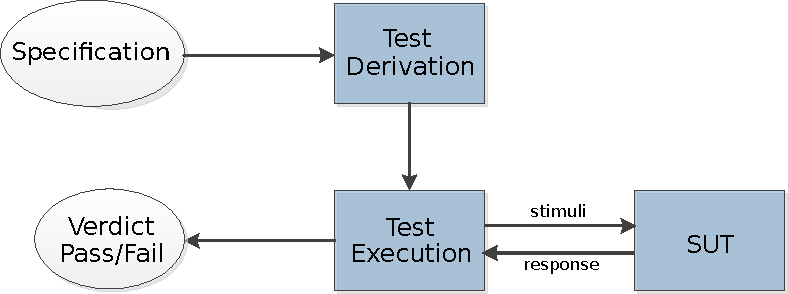
\includegraphics[width=0.75\textwidth]{model-based-testing.pdf}
  \end{center}
  \caption{A general model-based testing setup}
  \label{fig:model_based_testing}
\end{figure}

This type of model-based testing is called \textit{batch testing} or \textit{offline testing}. Another type of model-based testing is \textit{on the fly} testing. The main difference is that no test cases are derived, instead a transition in the model is chosen and tested on the system directly. The general architecture for this process is shown in Figure~\ref{fig:model_based_testing_on_the_fly}. A tool for on-the-fly testing is TorX~\cite{Tretmans:TorX}, which integrates automatic test generation, test execution, and test analysis. A version of this tool written in Java under continuous development is JTorX~\cite{Belinfante:JTorX}.

\begin{figure}[ht]
  \begin{center}
    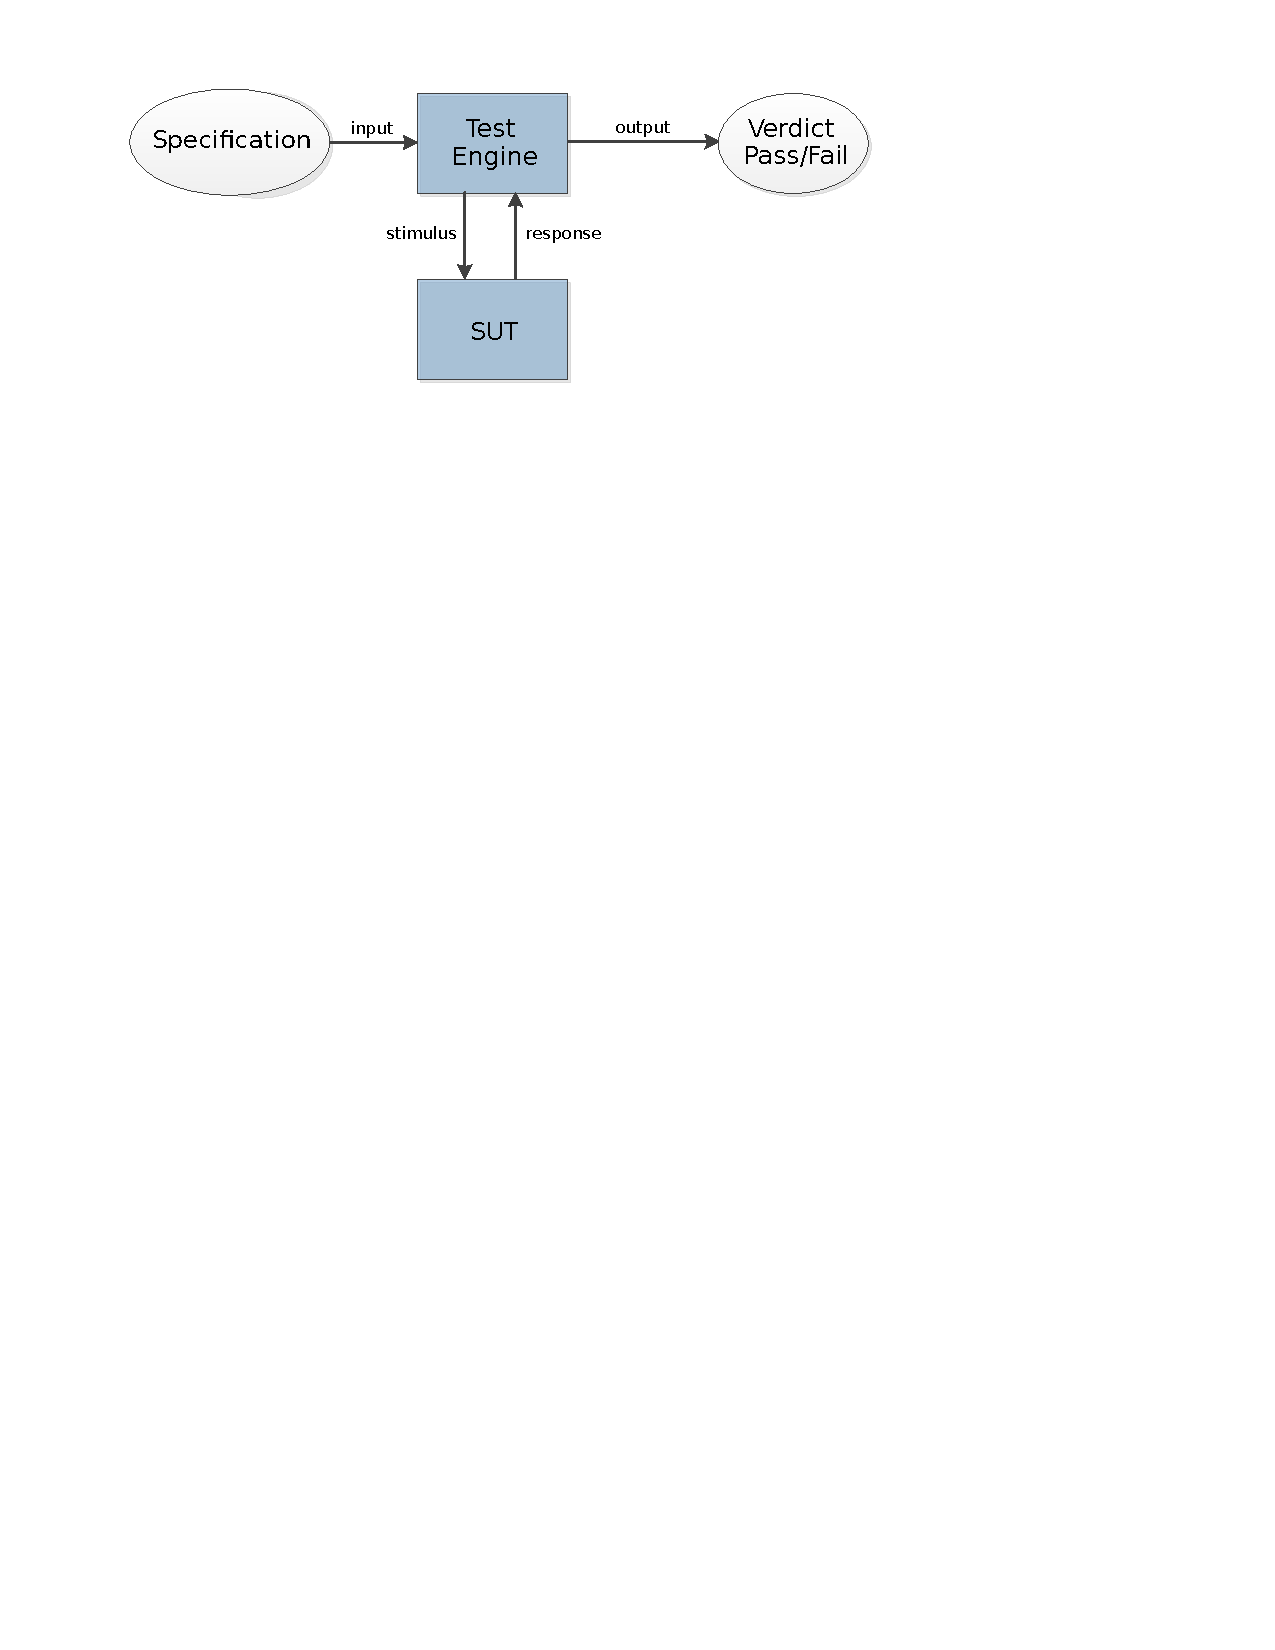
\includegraphics[width=0.75\textwidth]{mbt-on-the-fly.pdf}
  \end{center}
  \caption{A general 'on-the-fly' model-based testing setup}
  \label{fig:model_based_testing_on_the_fly}
\end{figure}

Variations of state machines and transition systems have been widely used as the underlying model for test generation. Other tools use the structure of data types to generate test data. First, previous work on model-based testing is given. Then, two types of models are introduced. These are basic formalisms useful to understand the models in the rest of the paper. Finally, the notion of \textit{coverage} is explained.

\subsection{Previous work}
Formal testing theory was introduced by De Nicola et al.~\cite{denicola:testing}. The input-output behavior of processes is investigated by series of tests. Two processes are considered equivalent if they pass exactly the same set of tests. This testing theory was first used in algorithms for automatic test generation by Brinksma~\cite{brinksma:testgeneration}. This led to the so-called \textit{canonical tester} theory. Tretmans gives a formal approach to protocol conformance testing (whether a protocol conforms to its specifications) in~\cite{Tretmans:conformancetesting} and an algorithm for deriving a sound and exhaustive test suite from a specification in~\cite{Tretmans:testgeneration}. A good overview of model-based testing theory and past research is given in "Model-Based Testing of Reactive Systems"~\cite{Broy:ModelBasedTesting}.

\subsection{Labelled Transition Systems}
A labelled transition system is a structure consisting of states with labelled transitions between them.

\begin{definition}
A labelled transition system is a 4-tuple	$\langle Q, L, T, q0\rangle$, where:
\begin{itemize}
\item $Q$ is a finite, non-empty set of states
\item $L$ is a finite set of labels
\item $T \in Q \times (L \cup \{\tau\}) \times Q$, with $\tau \notin L$, is the transition relation
\item $q0 \in Q$ is the initial state.
\end{itemize}
We write $q \xrightarrow{\mu}q'$ if there is a transition labelled $\mu$ from state q to state q', i.e., $(q, \mu, q') \in T$. The informal idea of such a transition is that when the system is in state $q$ it may perform action $\mu$, and go to state $q'$. 
\end{definition}

\subsection{Input-Output Transition Systems}
A useful type of transition system for model-based testing is the Input-Output Transition System (IOTS) by Tretmans~\cite{Tretmans:testgeneration}. Assuming that implementations communicate with their environment via inputs and outputs, this formalism is useful for describing system behavior. IOTSs have the same definition as LTSs with one addition: each label $l \in L$ has a type $t \in T$, where $T = \{input, output\}$. Each label can therefore specify whether the action represented by the label is a possible input or an expected output of the system under test.

An example of such an IOTS is shown in Figure~\ref{fig:iots_example}. This system allows an input of 20 or 50 cents and then outputs tea or coffee accordingly. The inputs are preceded by a question mark, the outputs are preceded by an exclamation mark. This system is a specification of a coffee machine. A test case can also be described by an IOTS with special pass and fail states. A test case for the coffee machine is given in Figure~\ref{fig:iots_test}. The test case shows that when an input of '50c' is done, an output of 'coffee' is expected from the tested system, as this results in a 'pass' verdict. When the system responds with 'tea', the test case results in a 'fail' verdict. The pass and fail verdicts are two special states in the test case, which are sink states, i.e., once in either of those the test case cannot leave that state. 

Test cases should always reach a pass or fail state within finite time. This requirement ensures that the testing process halts.
\begin{figure}[ht]
  \begin{center}
    \subfloat[An IOTS]{\label{fig:iots_example}$\xymatrix{
    \bullet \ar[r]^{?50c} \ar[d]_{?20c} & \bullet \ar[d]^{\mathit{!coffee}} \\
    \bullet \ar[r]_{!tea}       & \bullet }$
}
    \subfloat[An IOTS test case]{\label{fig:iots_test}$\xymatrix{
    \bullet \ar[r]^{!50c} & \bullet \ar[r]^{\mathit{?coffee}} \ar[d]_{?tea} & {pass}\\
    & {fail}}$}
  \end{center}
  \caption{The specification of a coffee machine and a test case as an IOTS}
\end{figure}

\subsection{Coverage}\label{sec:coverage}
The number of tests that can be generated from a model is potentially infinite. Therefore, there must be a test selection strategy to maximize the quality of the tests while minimizing the time spent testing. Coverage statistics help with test selection. Such statistics indicate how much of the SUT is tested. When the SUT is a black-box, typical coverage metrics are state and transition coverage of the model~\cite{Lee:testing, Nachmanson:testing, Hasan:testing}.

As an example, let us calculate the coverage metrics of the IOTS test case example in~\ref{fig:iots_test}. The test case tests one path through the specification and passes through 3 out of 4 states and 2 out of 4 transitions. The state coverage is therefore 75\% and the transition coverage is 50\%.

Coverage statistics are calculated to indicate how adequately the testing has been performed~\cite{Zhu:coverage}. These statisics are therefore useful metrics for communicating how much of a system is tested.

